\documentclass[a4paper,11pt,uplatex]{jsarticle}


% 数式
\usepackage{amsmath,amsfonts}
\usepackage{bm}
\usepackage{physics}
% 画像
\usepackage[dvipdfmx]{graphicx}
\usepackage[dvipdfmx,colorlinks=true,linkcolor=blue]{hyperref}
\usepackage{pxjahyper}
% リンク
\usepackage{url}

\begin{document}


\section{Small Experiment}
\subsection*{setup}
\subsubsection*{grating}
\url{https://www.thorlabs.co.jp/thorproduct.cfm?partnumber=GR25-1204}
\begin{table}[h]
\centering
\begin{tabular}{c|c}
  blaze wavelenght & 400 nm \\
  groove & 1200 \\
  blaze angle & 13$^\circ$53$^{'}$ \\
  dispeersion & 0.81 nm/rad
\end{tabular}
\end{table}

\subsubsection*{laser}
\url{https://www.thorlabs.co.jp/newgrouppage9.cfm?objectgroup_id=12994}
\subsubsection*{camera}
Toshiba Teli BU238MC F\\
\url{https://www.toshiba-teli.co.jp/products/industrial-camera/usb-camera-bu238m.htm}
\begin{table}[h]
\centering
\begin{tabular}{c|c}
  画素数 & 230万\\
  解像度 & 1920(H) x 1200(V)\\
  画素サイズ & 5.86 u x 5.86 u\\
  面積 & 11.25 mm x 7.03 mm 
\end{tabular}
\end{table}
\begin{figure}[tb]
  \centering
  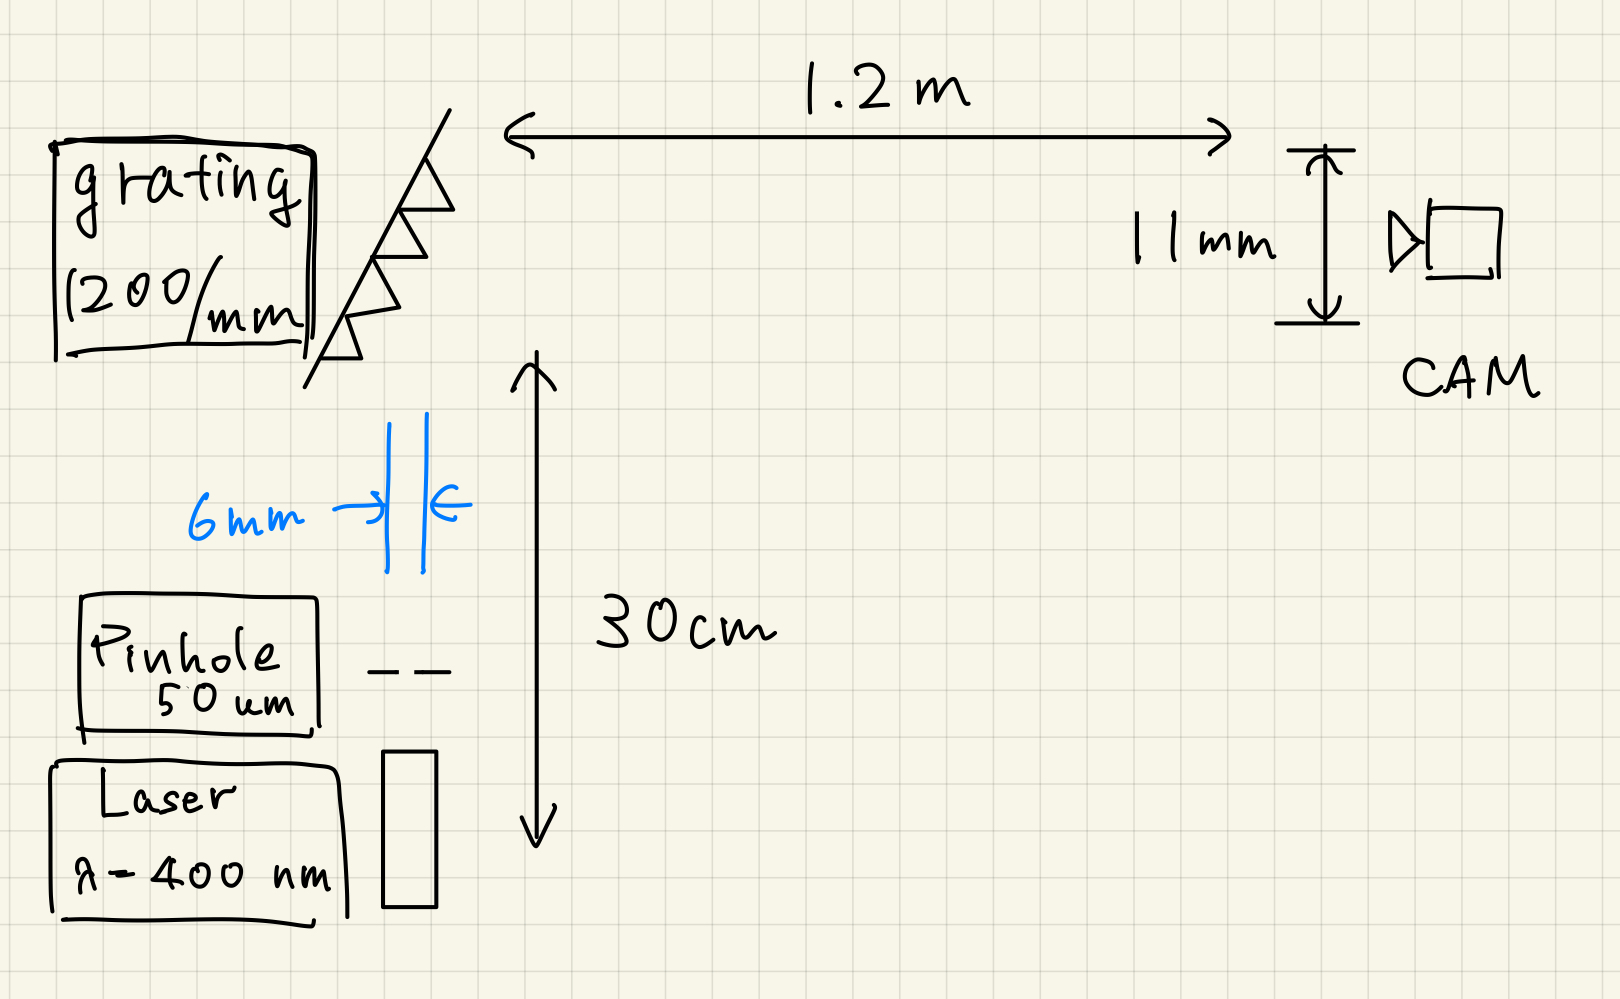
\includegraphics[width=0.8\linewidth]{image/SE-1.jpeg}\\
  \caption{}
  \label{}
\end{figure}
\begin{figure}[tb]
  \centering
  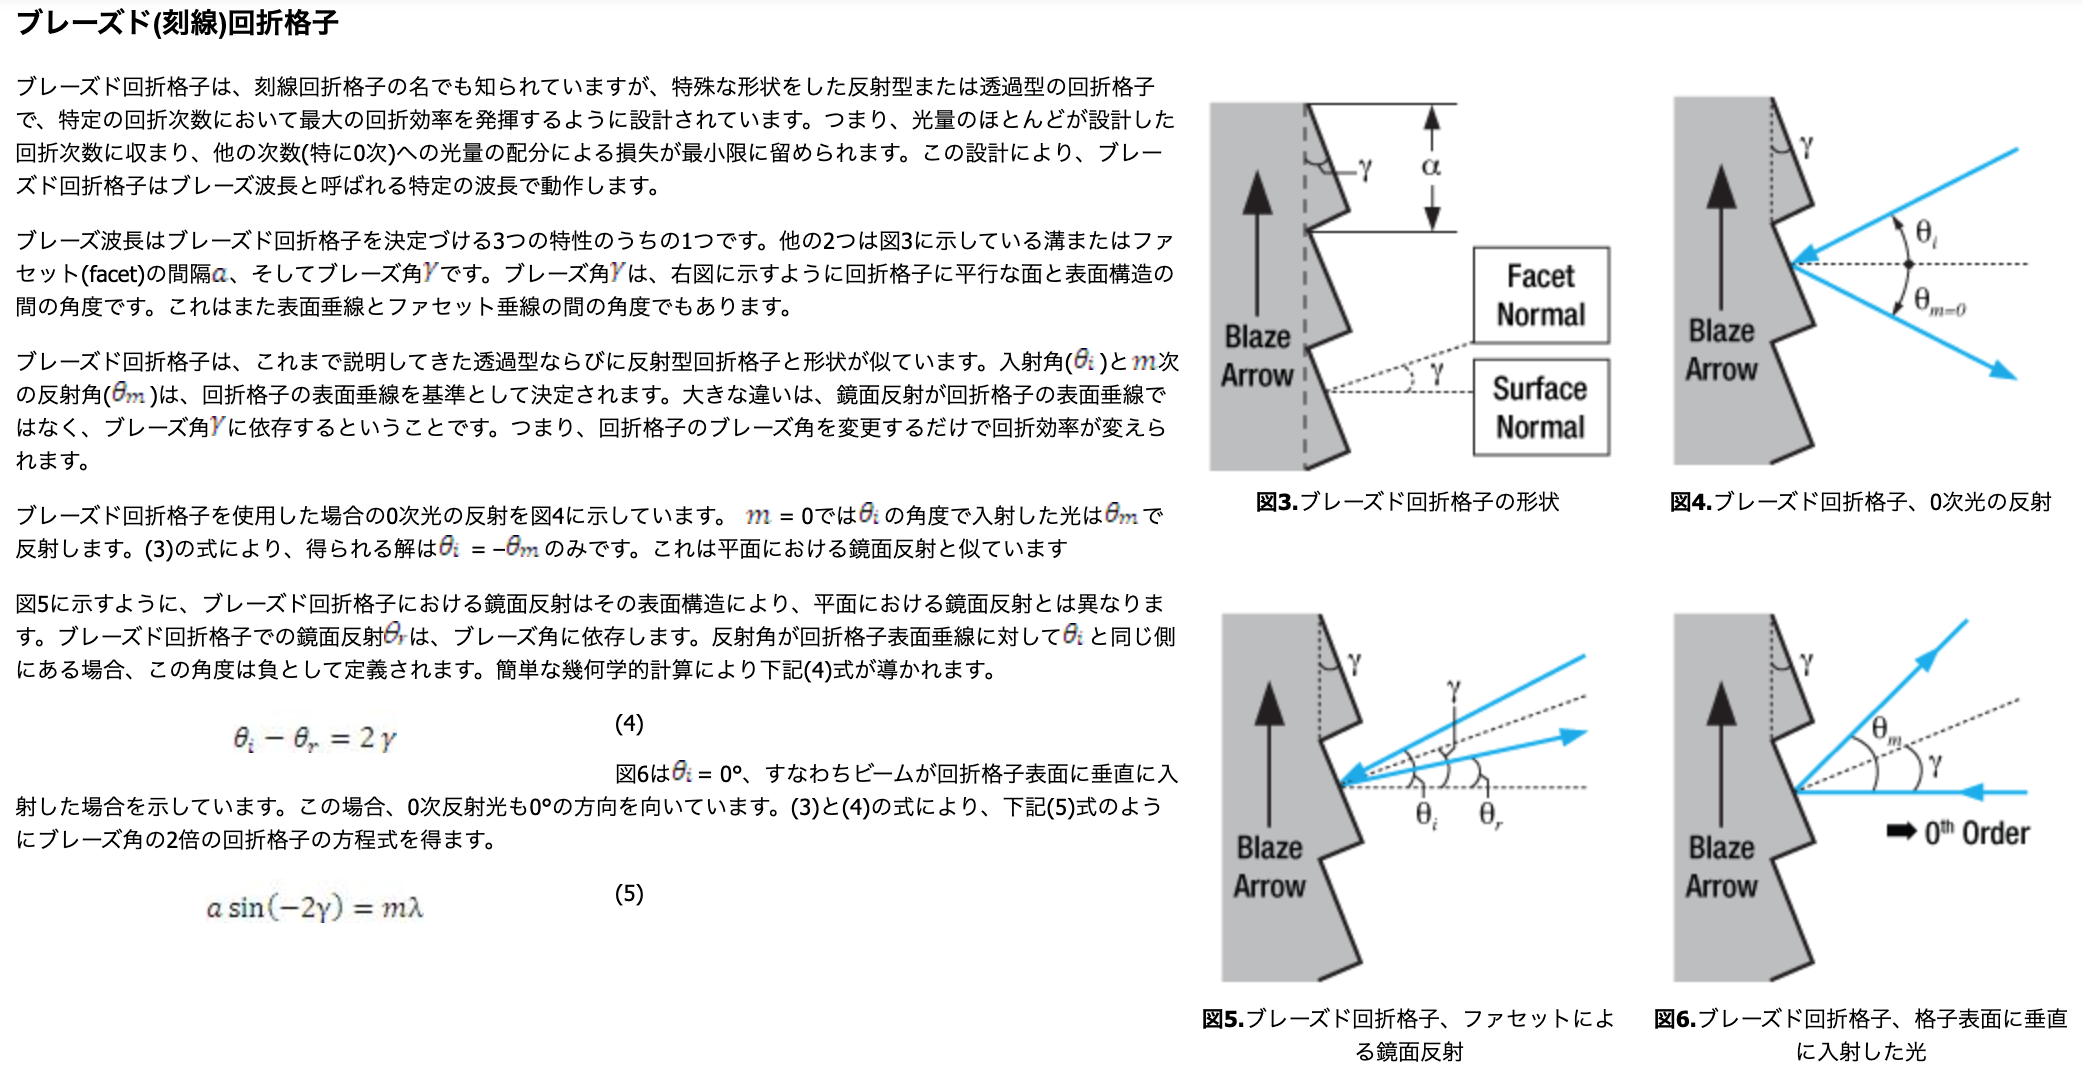
\includegraphics[width=0.8\linewidth]{image/SE-2.png}\\
  \caption{}
  \label{}
\end{figure}









\clearpage

\begin{figure}[tb]
  \centering
  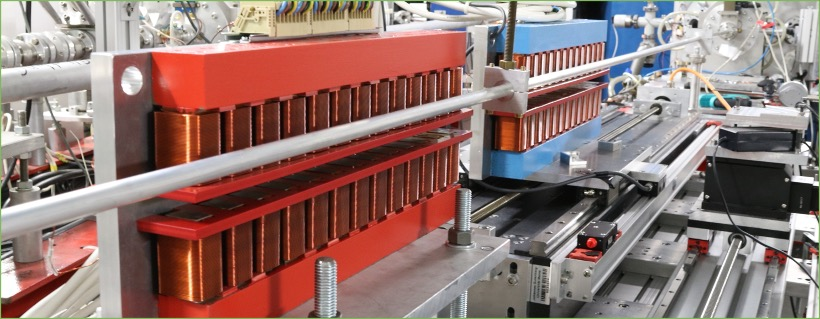
\includegraphics[width=0.8\linewidth]{image/1-1.jpg}\\
  \caption{サンプルの図}
  \label{sample_image}
\end{figure}

\begin{itemize}
  \item a
\end{itemize}
\begin{enumerate}
  \item b
\end{enumerate}

\begin{align}
\frac{1}{2} = \qty(\frac{1}{3}) + \qty{1}\Sigma
\end{align}
\end{document}